\documentclass[a4paper,10pt]{article}
\usepackage[utf8]{inputenc}
\usepackage[T1]{fontenc}	
\usepackage[italian]{babel}

\usepackage{amsmath}
\usepackage{amsfonts}
\usepackage{amssymb}
\usepackage{graphicx}

\usepackage[left=2cm,right=2cm,top=2cm,bottom=2cm]{geometry}
\geometry{a4paper}

\usepackage{booktabs}
\usepackage{verbatim}
\usepackage{subfig}

\usepackage[cdot, thickqspace, squaren]{SIunits}
\usepackage{float}

% macro
\def\code#1{\texttt{#1}}

\title{Esperienza di Ottica 2}
\author{Gruppo BL \\ Candido Alessandro, Luzio Andrea, Mazziotti Fabrizio}

\begin{document}

\maketitle

\section{Scopo}
L'esperienza è divisa in due parti:
\begin{itemize}
	\item nella prima parte si vuole misurare la lunghezza d'onda di un laser ad He-Ne.
	\item nella seconda parte si vuole misurare la lunghezza d'onda della radiazione emessa da una lampada al mercurio.
\end{itemize}

\section{Esperienza A: Misura della lunghezza d'onda di un laser ad He-Ne}

\subsection{Strumentazione}

\begin{itemize}
	\item Spettroscopio a prisma:
	\item Laser ad He-Ne;
	\item Schermo per visualizzare la figura di diffrazione;
	\item Specchio per deviare il raggio laser sullo schermo;
	\item Righello graduato di un calibro ventesimale;
	\item Riga;
	\item Torcia.
\end{itemize}

\subsection{Misura della lunghezza d'onda del laser ad He-Ne}
In questa prima parte dell'esperienza si vuole misurare la lunghezza d'onda di un laser ad He-Ne. Per fare ciò si è indirizzato il laser, attraverso uno specchio, sulla scala graduata di un calibro ventesimale, utilizzando queste tacche come un reticolo di diffrazione. Poiché il passo $d$ di questo reticolo( d = 1 mm) è molto più grande della lunghezza d'onda attesa ($\lambda_{att} \sim$ 650 nm), si è fatto in modo che il fascio laser incida sul righello con un angolo di circa $\pi/2$, altrimenti non si avrebbe modo di apprezzare la figura di diffrazione.
Tale figura si può osservare su un opportuno schermo vicino al banco di lavoro su cui è fissato un foglio di carta per la presa dati.

L'equazione che lega la posizione dei massimi di diffrazione al passo reticolare $d$ e all'angolo di incidenza $\theta_i$ è la seguente:

\begin{equation}
d(sin\theta_i - sin\theta_d)= m\lambda
\label{reticolo}
\end{equation}

dove $\theta_d$ è l'angolo di riflessione.

Una rappresentazione schematica di ciò che accade è mostrata in \figurename{~\ref{fig:espa}.

\begin{figure}[H]
	\centering
	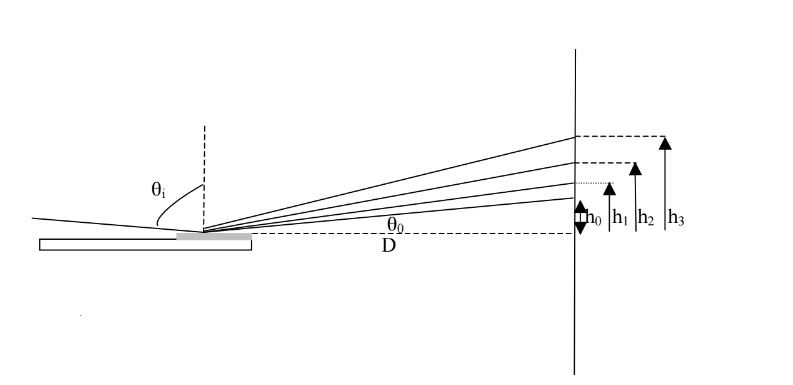
\includegraphics[width=0.7\textwidth]{../grafici/espa.png}
	\caption{Schema di un raggio incidente sul calibro e della figura di diffrazione che si viene a formare. $\theta_i$ è l'angolo di incidenza, D la distanza del reticolo dallo schermo, $\theta_n$ e $h_n$ sono rispettivamente il complementare dell'angolo di riflessione e la distanza dei vari massimi dalla quota del calibro sullo schermo.}
	\label{fig:espa}
\end{figure}

Per prima cosa si è trovata sullo schermo la quota del calibro, poiché tutte gli ordini di diffrazione devono essere riferiti a questa misura che rappresenta lo zero sull'asse dello schermo. Tale quota si è trovata misurando il punto intermedio tra la luce non riflessa dal calibro (cioè quella che si vede in assenza di esso) e l'ordine zero di diffrazione (cioè la riflessione geometrica), che nella figura \figurename{~\ref{fig:espa} corrisponde alla quota $h_0$. Inoltre dalla posizione dell'ordine zero (m = 0), utilizzando la formula \eqref{reticolo}, si può trovare l'angolo di incidenza $\theta_i$.
	
Successivamente si sono presi gli altri ordini e, dalla misura della distanza di essi dallo zero dell'asse precedentemente trovato ($h_n$), si sono trovati i complementari degli angoli di riflessione utilizzando le formule

\begin{equation}
sin\theta_{d,n} = sin(\pi/2 - \theta_n)
\label{thetad}
\end{equation}
\begin{equation}
\theta_n = arctg(h_n/D)
\label{thetan}
\end{equation}

dove D è la distanza del calibro dallo schermo, misurata mediante un metro a nastro.
\paragraph{Errori}
Per quanto riguarda gli errori associati alle misure, si sono effettuati i seguenti accorgimenti:
\begin{itemize}
\item Per ogni misura effettuata con il metro a nastro per le lunghezze sullo schermo relative agli ordini di diffrazione si sono presi gli estremi delle bande luminose (quelle verticali,
%\footnote{Nella parte superiore di ogni banda era presente un alone con luminosità decrescente che non si è considerato per l'acquisizione dati, mentre nella parte inferiore della banda questo alone non era presente. L'alone probabilmente è dovuto alla non perfetta monocromaticità del fascio laser, mentre si ritiene che la mancanza dell'alone nella parte inferiore sia dovuta al fatto che le tacche del calibro sono in rilievo}
%non lo so, ho sparato, se avete altre idee proponete
quelle orizzontali sono dovute solo alla larghezza del fascio) che contraddistinguono tale punto e si è considerata come valore la semisomma e come errore (massimo) la semidifferenza tra questi punti.
%non abbiamo fatto così ma altrimenti dovrei scrivere " abbiamo preso un punto a caso al "centro" della banda e poi gli estremi", che è brutto. Comunque il risultato non cambierebbe di tanto quindi io lascierei cosi.
\item Per la distanza D dello schermo dal calibro, poiché lo spot del laser sul calibro è allungato, si sono identificate 3 misure: una tra lo schermo e la zona in cui il fascio laser aveva la maggior luminosità sul calibro e le altre due dallo schermo fino agli estremi di luminosità del laser sempre sul calibro. Si è quindi deciso di considerare come effettiva distanza D la media delle tre misure, mentre per stimare l'errore associato si è usata la deviazione standard delle tre misure. I valori ottenuti per queste 3 misure sono riportati in \tablename{~\ref{tab:D}}. Da questi dati si è ottenuto $D = 210 \pm 5 cm$.
%Non ha alcun senso questa roba!

\begin{table}[H]
	\centering
	\begin{tabular}{c|c|c}
\hline
205.0$\pm$0.1 & 210.1$\pm$0.1 & 214.7$\pm$0.1\\
\hline
	\end{tabular}
\caption{Distanze caratteristiche schermo-calibro espresse in cm. La misura centrale è quella che si è assunta come D, mentre le altre due servono per stimare l'errore.}
\label{tab:D}
\end{table}

\item Gli errori associati agli angoli si sono ottenuti, propagando attraverso le formule \eqref{thetad} e \eqref{thetan}, gli errori ottenuti per    la distanza dello schermo dal calibro (D) e per i vari ordini di diffrazione ($h_n$).
\end{itemize}

\paragraph{Risultati analisi dati}
Si è ottenuto come angolo di incidenza $\theta_i = (88.10 \pm 0.05)\degree$, risultato molto vicino a $90\degree$, come ci si poteva aspettare in seguito alle condizioni in cui ci si è posti per l'esperienza. I vari valori delle altezza $h_n$ rispetto allo zero dello schermo e dei seni degli angoli di riflessione sono riportati in \tablename{~\ref{tab:data}.

\begin{table}[H]
	\centering
	\begin{tabular}{c|c|c|c|c}
x[cm] & dx[cm] & ordine & $\theta_d[\degree]$ & d$\theta_d[\degree]$ \\
\hline
6.95 & 0.07 & 0 & 88.0677 & 0.0007 \\
10.2 & 0.1 & 1 & 87.179 & 0.002 \\
12.6 & 0.2 & 2 & 86.514 & 0.004 \\
14.7 & 0.1 & 3 & 85.932 & 0.002 \\
16.5 & 0.2 & 4 & 85.434 & 0.004 \\
18.1 & 0.2 & 5 & 84.993 & 0.005 \\
19.6 & 0.2 & 6 & 84.579 & 0.006 \\
21.0 & 0.2 & 7 & 84.193 & 0.006 \\
22.3 & 0.2 & 8 & 83.835 & 0.006 \\
23.5 & 0.2 & 9 & 83.506 & 0.007 \\
24.7 & 0.2 & 10 & 83.176 & 0.007 \\
25.8 & 0.2 & 11 & 82.88 & 0.01 \\
26.9 & 0.3 & 12 & 82.57 & 0.01 \\
27.9 & 0.3 & 13 & 82.30 & 0.01 \\
29.0 & 0.3 & 14 & 82.00 & 0.01 \\
30.0 & 0.3 & 15 & 81.73 & 0.01 \\
30.9 & 0.3 & 16 & 81.48 & 0.01 \\
	\end{tabular}
\caption{Dati raccolti per i vari ordini di diffrazione e valore del seno degli angoli di riflessione. La variabile x con il suo errore dx rappresenta la distanza dei vari massimi di diffrazione dallo zero sull'asse dello schermo.}
\label{tab:data}
\end{table}



Riscrivendo l'equazione \eqref{reticolo} come:

\begin{align*}
sin\theta_d = - m(\lambda/d) + sin\theta_i
\end{align*} 
  
si è effettuato un fit lineare utilizzando come variabile dipendente $\sin\theta_d$ e come variabile indipendente $m$. Il grafico è riportato in \figurename{~\ref{fig:fita}.
Dal valore $d$ del passo reticolare del calibro si è quindi ottenuta una misura della lunghezza d'onda del laser ad He-Ne, mentre l'intercetta è proprio $\sin\theta_i$. I valori ottenuti sono riportati in \tablename{~\ref{tab:fita}}.


\begin{table}[H]
	\centering
	\begin{tabular}{c|c|c|c}
$\lambda$[nm] &$\lambda_{atteso}$ &$\theta_i[\degree]$& $\chi^2/ndof$ \\
\hline
627$\pm$10 & 650 & 88.11$\pm$0.04 & 0.1/15\\
\hline
	\end{tabular}
\caption{Risultati del fit lineare.}
\label{tab:fita}
\end{table}


\begin{figure}[H]
	\centering
	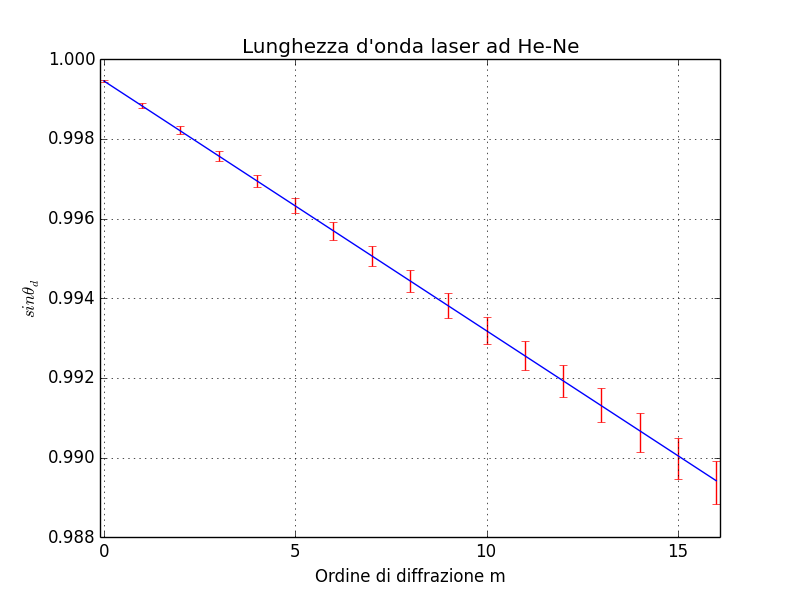
\includegraphics[width=0.7\textwidth]{../grafici/fita.png}
	\caption{Fit lineare dell'angolo di diffrazione $sin\theta_d$ in funzione dell'ordine di diffrazione m.}
	\label{fig:fita}
\end{figure}


Dai risultati del fit si può osservare come il valore di $\theta_i$ sia compatibile con la misura effettuata precedentemente e con le condizioni scelte nell'esperienza riguardo quest'angolo.
Il valore della lunghezza d'onda del laser ad He-Ne è dell'ordine del valore atteso (650 nm), compatibile entro 2$\sigma$.

%Tuttavia si è notato come la misura della distanza schermo-calibro influisca significativamente sul risultato ottenuto per $\lambda$, infatti cambiando la misura scelta per D di 2-3cm (sempre all'interno degli estremi riportati in \tablename{~\ref{tab:D}}), la lunghezza d'onda varia di $\sim 20nm$. Questo induce a pensare che effettivamente il punto a maggior luminosità sul calibro si discosti di un po' da quello considerato.
% io lo ho scritto, fatemi sapere se secondo voi ce la dobbiamo mettere questa cosa.

Il $\chi^2$ è molto minore della media. Ciò è dovuto al fatto che tutti gli errori considerati nell'elaborazione dati sono errori strumentali e non statistici, che quindi risultano essere inevitabilmente una sovrastima dell'errore da attribuire alla misura per effettuare il fit.

 

\section{Esperienza B: Interferometro di Michelson}

\subsection{Strumentazione}

\begin{itemize}
	\item Inteferometro di Michelson;
	\begin{itemize}
		\item spaziatore in alluminio;
		\item punta di riferimento per contare i massimi;
		\item filtro verde;		
	\end{itemize}
	\item Laser ad He-Ne;
	\item Lampada al Mercurio
	\item Schermo per visualizzare la figura di interferenza;
	\item Riga;
	\item Torcia.
\end{itemize}

\begin{figure}[H]
	\centering
	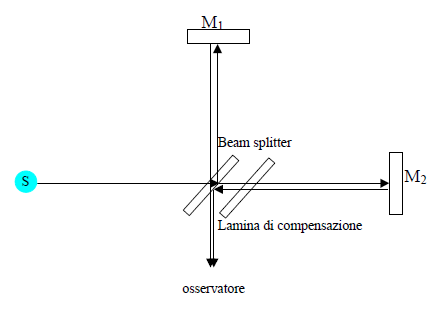
\includegraphics[width=0.7\textwidth]{../grafici/MichelsonMorley.png}
	\caption{Schema dell'interferometro di Michelson e Morley}
	\label{fig:MMint}
\end{figure}

\subsection{Misura del fattore di demoltiplica della leva micrometrica}
Per misurare il fattore di demoltiplica della leva si è acceso il laser ad He-Ne e si è posizionato come sorgente dell'interferometro.
Si è quindi posizionato lo specchio M$_2$, agendo opportunamente sulle viti relative, in modo da visualizzare le frange di interferenza al centro dello schermo, posto a distanza e ortogonale al fascio uscente.

Una volta trovata la configurazione di visualizzazione delle frange si è ruotato il micrometro relativo allo specchio M$_1$ di $20 \pm 0.5~$\footnote{L'errore sulla misura delle tacche è stato posto pari al quarto di tacca, poiché si è ritenuto che le tacche fossero sufficientemente spaziate da apprezzarlo. Essendo la misura una differenza con la posizione dello 0, anch'essa affetta da incertezza, si ottiene come errore la mezza tacca.} tacche, filmando lo schermo sul quale scorrevano le frange.

Si è dunque riprodotto il video rallentato e si sono contate le frange passate nella rotazione eseguita del micrometro, ottenendo un valore di $110 \pm 1$ frange. L'errore in questo caso è dovuto all'incertezza sulla posizione dell'ultima frangia osservata rispetto alla prima.

\subparagraph{Errore sul numero delle frange} Si sarebbe potuta ottenere una migliore stima dell'errore osservando nel video la posizione della frangia iniziale e finale osservate, però a questo punto sarebbero intervenute altre fonti di incertezza, come il fatto che le frange hanno un profilo variabile e non nettamente definito e il fatto che la posizione della fotocamera che ha ripreso le frange non era fissata e costante. Si è quindi deciso di porre l'incertezza pari a una frangia, anche se questo è una leggera sovrastima dell'incertezza reale.

\subparagraph{Fattore di demoltiplica} Si è infine trovato un fattore di demoltiplica pari a $\unit{1.74 \pm 0.05}{\micro\meter / tacca}$.

\subsection{Misura della lunghezza d'onda del mercurio}
Per la misura della lunghezza d'onda della riga verde del mercurio si è sostituito il laser a He-Ne, inserito nella misura precedente, con una lampada a mercurio, e si è interposto un filtro verde di fronte alla lampada, in modo da selezionare la componente spettrale d'interesse.

Si è riposizionato lo specchio M$_2$, sempre agendo sulle apposite viti, in modo da visualizzare le frange d'interferenza.

Poiché la luce emessa era d'intensità notevolmente minore rispetto a quella del laser non si è potuto visualizzare sullo schermo la figura d'interferenza. Si è cercato di filmare ugualmente il fascio uscente dall'interferometro, ma non si è riusciti ad ottenere un risultato adeguato ad una misura delle frange come nel caso precedente. Si è dunque proceduto con un'osservazione diretta delle frange.

Si è dunque posizionata una punta di riferimento sul filtro, in modo da aiutare a distinguire le frange nell'osservazione diretta. Data la sensibilità del micrometro e la difficoltà nell'identificazione esatta delle frange successive quando in moto, si è deciso di ripetere la misura più volte, con osservatori diversi, per ridurre l'incertezza statistica.

\subparagraph{Lunghezza d'onda Hg} Si è ottenuto infine che in $\unit{4 \pm 0.5}{tacche}$ sono passate $\unit{30 \pm 5}{frange}$, da cui si ha una misura della lunghezza d'onda del mercurio pari a $\unit{470 \pm 90}{\nano\meter}$, compatibile con il valore noto di $\unit{546}{\nano\meter}$.

Si è ottenuta una misura con un'incertezza del $20\%$, questo è dovuto all'entità dell'errore nel conteggio del numero di frange da parte degli osservatori, che non si è riusciti operativamente a limitare.

\subsection{Visualizzazione delle frange di interferenza con luce bianca}

Per visualizzare le frange di interferenza della luce bianca è stato necessario rendere più corto il braccio dello specchio $M_1$ in modo che i cammini ottici fossero uguali.

Si hanno fenomeni di interferenza perché la condizione per avere un massimo, appunto quando i due bracci dello strumento sono uguali, è soddisfatta per tutte le lunghezze d'onda simultaneamente. Quando i due bracci hanno lunghezze diverse componenti con lunghezze d'onda simili prendono fasi molto diverse e dunque regioni molto vicine dello spettro sono in interferenza costruttiva o distruttiva, facendo si che si veda semplicemente luce bianca.\footnote{La differenza di fase fra i due bracci ad una data lunghezza d'onda è $\phi = \Delta D/(2\pi\lambda)$ dunque $d\phi=\delta D/(2\pi\lambda)d\lambda/\lambda$ dunque per una differenza di lunghezza d'onda di un solo $10 nm$  per una lunghezza d'onda del verde si ha per una differenza fase di $\pi [rad]$ con una differenza di cammino di circa $0.25 mm$.}

Diversamente per $\Delta D=0$ tutte le componenti sono in interferenza costruttiva, mentre spostandosi poco da questa condizione ampie zone dello spettro visibile vanno in interferenza distruttiva lasciando visibili solo certi colori. Questo dovrebbe causare la marcata opalescenza osservata. Non è stato possibile prendere immagini di tale osservazione per la poca luminosità dello strumento.

\end{document}